\section{The binomial distribution} \label{s2} 

\ssn{Learning outcomes}
After studying this week you will be able to: 
\begin{itemize}
\item use the Binomial distribution to compute probabilities;
\item use probability generating functions to compute probabilities is some simple examples. 
\item explain the importance of ``independence'' and determine whether some simple random variables are independent. 
\end{itemize}
\end{n}  

\subsection{Preparation for the week} 

\ssn{Motivating problem} \label{mp2}
A production line produces components and it is assumed that on any given day, each component independently has a probability $p$ of being faulty. It is hoped that no more than 5\% are faulty, in other words that $p \leq 0.05$.
Ten random samples are taken of the product each day and if two or more are faulty then an incident report is filed and the cause investigated.  If in fact exactly 5\% are faulty, how likely is it that on a given day an incident report is filed? 
\end{n}

\ssn{A generalisation}
Let us consider a general version of the problem.  Supposing we have a process that each time it is carried out produces a ``success'' (S) with probability $p$ or a failure (F) with probability $q=1-p$. In the example above, success could be finding a faulty example; in another case it might be rolling a `6' with a D6.  We are assuming that each execution of the process is ``independent'', meaning that its success or failure  each time is not influenced by what might have happened before.  If we now repeat this process $n$ times, what is the probability that we get exactly $k$ successes? 

If, for example, $n=8$ and $k=3$, then one particular sequence of successes and failures is $SSFFSFFF$. Thinking of a large probability tree, the probability of this exact sequence is 
 \[
    ppqqpqqq = p^3 q^5 = p^k q^{n-k}. 
\]
How many other sequences of eight S's and F's are there with precisely three S's?  That is the same question as asking how many ways are there of choosing three things from eight.  It is the Binomial coefficient 
 \[
       \binom 83 = \frac{8!}{3! \, 5!}. 
  \]
Adding all these possibilities, the probability of three successes in eight trials is exactly 
  \[
     \binom 83 p^k q^{n-k}. 
  \]
For the general problem, the probability of $k$ successes in $n$ trials is therefore 
  \[
       \PP( \text{$k$ successes}) =  \binom nk p^k q^{n-k} =  \frac{n!}{k! \, (n-k)!} p^k q^{n-k}. 
  \]
 A random variable with probabilities given by this formula is called a \emph{Binomial random variable with parameters $n,p$}.  It is a fundamentally important example.  
\end{n}

\ssn{Example}
I roll a D6 twelve times.  How likely is it that I roll precisely two sixes?   Here, $n=12, k=2$ and $p=1/6$. So the answer is 
 \[
    \binom{12}2 \left(\frac{1}{6}\right)^2  \left(\frac{5}{6}\right)^{10}
     \approx 0.296.
 \]
\end{n}

\sse{Exercise}
I toss a fair coin 6 times.  How likely is it that I roll $k$ heads where $k=0,1,2,3,4,5,6$? 
\end{e}
\sss 
Use the formula with $n=6$ and $p=1/2$.  For instance, $\PP(k=3) = 20/64 = 5/16$. 
\end{s}

\ssn{Solution to motivating problem}
If we think of finding a faulty item in \S\ref{mp2} as a ``success'', then for the factory problem we have $p=0.05$ and $n=10$.  We first calculate the probability of not generating an incident report, i.e.\ of fewer than two successes or equivalently $k=0$ or $k=1$.   

The probability of $k=0$ successes is
 \[ 
     \binom{10}{0} p^0 q^{10}  = 0.95^{10} = 0.5987
 \]
and the probability of $k=1$ successes is 
 \[
     \binom{10}{1}  p^1 q^{9} = 10 \,(0.95)^9 \, 0.05^1 = 0.3151
 \]
and so the probability two or more (and hence an incident report) is $1-0.5987-0.3151=0.0862$. 
\end{n}

\begin{table}{h} 
  \begin{tabular}{cc} 
    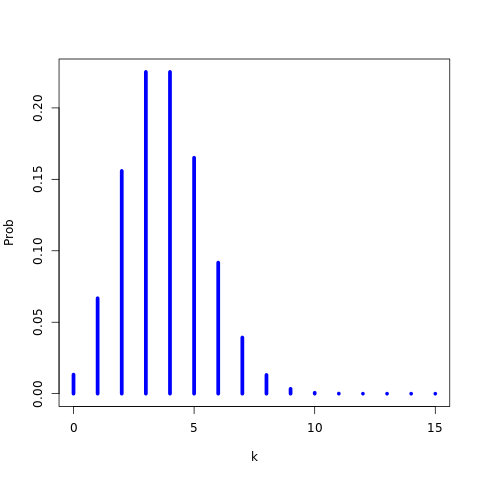
\includegraphics[width=0.45\textwidth]{images/binom15P25.png} & 
    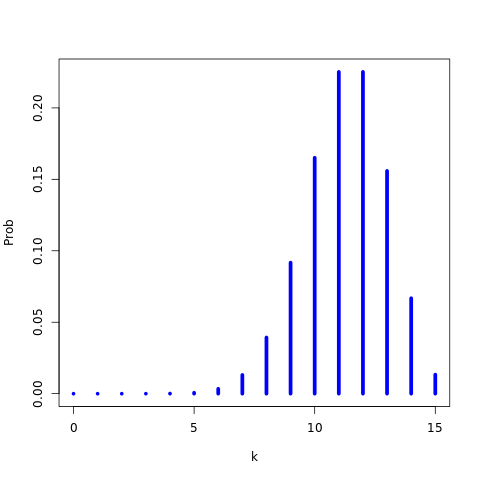
\includegraphics[width=0.45\textwidth]{images/binom15P75.png} \\
     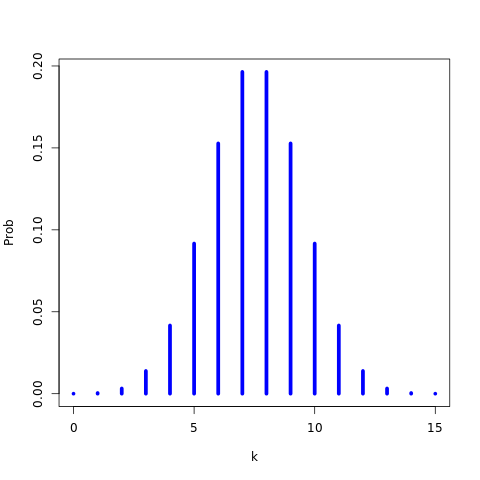
\includegraphics[width=0.45\textwidth]{images/binom15P5.png} & 
    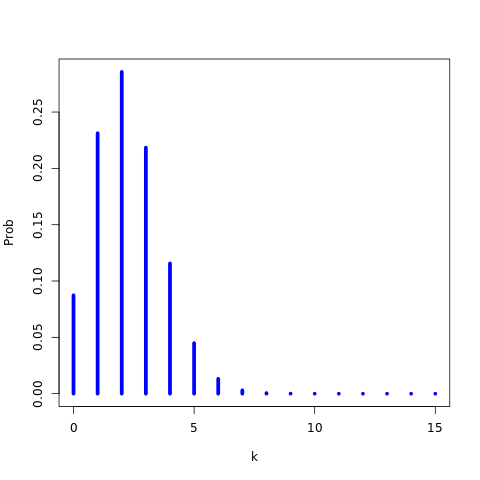
\includegraphics[width=0.45\textwidth]{images/binom15P15.png} \\
  \end{tabular}
 \caption{\label{binpics} Binomial with $n=15$ and $p=0.15, 0.25, 0.5, 0.75$ in some order}
\end{table}


\sse
In table~\ref{binpics} ``probability mass functions'' for Binomial distributions with different probabilities are plotted. The height of each vertical bar is the probability of the corresponding outcome. Which is which?
\end{e}

\sss
The top row has $p=0.25$ and $p=0.75$. Note the symmetry between them. 
The bottom two are $p=0.5$ (note the symmetry about its centre) and $p=0.15$. 
\end{s}


\sse 
An unprepared student takes a multiple choice test of 10 questions by guessing randomly which of the three possible answers to each question is correct. Use the Binomial distribution to find how likely is the student to get a grade A by scoring at least 7 out of 10. 

As an example to get you started, the probability of exactly four correct answers is 
 \[
    \binom{10}{4} \left( \frac13\right)^4 \left( \frac23 \right)^6 \approx 0.228. 
 \]
\end{e}

\sss
\[
    \binom{10}{7} \left( \frac13\right)^7 \left( \frac23 \right)^3 +  
    \binom{10}{8} \left( \frac13\right)^8 \left( \frac23 \right)^2 +  
    \binom{10}{9} \left( \frac13\right)^9 \left( \frac23 \right)^1 +  
    \binom{10}{10} \left( \frac13\right)^{10} \left( \frac23 \right)^0  \approx 0.019661636.
 \]
 (I give many decimal places because the e.g.\ leaving out the 1/10 possibility only affects the fifth decimal place!) 
\end{s}



\subsection{Notes} 


\ssn{Definitions and notation}
Let $X, Y$ be two random variables taking non-negative integer values. We say that $X$ and $Y$ are \emph{independent} if for all $k,l$ we have
 \[
     \PP( \text{$X=k$ and $Y=l$} ) \quad = \quad \PP( X=k) \, \PP(Y=l).
  \]
 \end{n}

\ssn{Examples}
\begin{enumerate}
\item Roll two D6 and let $X$ be the number on the first die and $Y$ be the number on the second.   Then 
 \[
 \PP( \text{$X=3$ and $Y=4$} ) = \frac{1}{36} = \frac16 \, \frac16 = \PP(X=3)\, \PP(Y=4)
 \]
 and similarly for all the other possibilities. So $X$ and $Y$ are independent. 
 \item Continuing the previous example, let $Z$ be the random variable which is the sum of the numbers on the two dice. Then 
  \[
    \PP(\text{$X=3$ and $Z=9$}) = \frac1{36} \quad \not = \quad \PP(X=3) \, \PP(Z=9) = \frac16 \, \frac19 = \frac{1}{54}. 
  \]
  These two random variables are not independent.  The point is that knowing that $X=3$ increases the probability that $Z=9$.   
 \end{enumerate}
\end{n}

\ssn{The ``probability generating function''}
Let $X$ be a binomial random variable  with parameters $n,p$ as above. We will in future often use the abbreviated notation ``Let $X \sim \bino(n,p)$'' for this.  Consider the polynomial  
 \[ 
    G_X(s) = ( ps+q)^n = \sum_{k=0}^n \binom nk p^k q^{n-k} s^k  
  \]
 where the expansion on the right-hand side is just the Binomial Theorem.\footnote{It is not as well know as it should be that Professor Moriarty, Sherlock Holmes' arch-enemy, was an expert on the Binomial Theorem.}    
 
 Comparing the coefficients in the expansion with the probabilities, we see that 
  \beq{gefun}
     G_X(s) = \sum_{k=0}^n \PP( X = k)\, s^k.  
  \eeq 
The polynomial whose coefficients encode the probabilities of a random variable taking integer values in this way is called the \emph{probability generating function (pgf)} of the random variable.  
\end{n}

\ssn{Comment} In the definition, it is tempting to ask what the variable $s$ ``is''. The answer is that it does not represent anything. It just turns out that the polynomial is a good way to represent or encode the random variable. 
\end{n} 

\ssn{Examples} Suppose $X$ is the result of rolling a single D4. Then the pgf for $X$ is 
 \[
      \frac{1}{4} s +  \frac{1}{4} s^2 + \frac{1}{4} s^3 + \frac{1}{4} s^4. 
 \]
Another example would be to let $Y$ be the number of H resulting from tossing two coins. This has generating function 
 \[
  G_Y(s) = \PP(Y=0) s^0 + \PP(Y=1) s^1 + \PP(Y=2) s^2 = 
     \frac14 + \frac12 s + \frac14 s^2.
 \]
 The latter example is in fact just the Binomial example with $n=2$ and $p=1/2$. 
 \end{n}

\ssn{Properties} 
The pgf $G_X(s)$ of the random variable $X$ has the properties: 
\begin{itemize}
\item $G_X(1) = 1$; 
\item $G_X'(1) = \EE(X)$, the expected value of $X$.  
\end{itemize}
\bpr
The first of these is immediate from the definition. for the second, differentiate Equation~(\ref{gefun}) above and then set $s=1$ to obtain 
 \[
      G'(1) = 1 p_1 + 2 p_2 + \dots + n p_n = \EE(X). 
 \]
\epr
\end{n}

\ssn{Proposition}
Let $X$ be a binomial random variable with parameters $n, p$.  Then the expected value $\EE(X) = np$. 
\begin{proof}
The generating function is $G_X(s) = ( ps+q )^n$. So $G_X'(s)= np(ps+q)^{n-1}$ and so $\EE(X) = G_X'(1) = np 1^{n-1} = np$. 
\end{proof}
\end{n}

\ssn{An example to work through}
Suppose now that we roll two D4 and let $Y$ denote the random variable which is the sum of the numbers showing on the two dice. We say that $Y$ is the \emph{sum} of random variables $X_1, X_2$ where $X_1, X_2$ are the numbers showing on the first and second die respectively. The two random variables $X_1, X_2$ are independent D4 random variables.  

Compute the probabilities that $Y$ takes each of the possible values $2,3,\dots,8$ and hence write down the generating function $G_Y(s)$ of $Y$. 

Now expand the expression which is the square of the D4 generating function 
\[
   (G_X(s))^2 =  \left( \frac{1}{4}(s+s^2+s^3+s^4) \right)^2.   
\]
You should discover that $G_Y(s)= (G_X(s))^2$. 

We see in this case that \emph{adding the two independent random variables corresponds to multiplying their generating functions.} We will prove this result later and understand the idea of ``independence'' better. 
\end{n}

\sse 
What is the probability of rolling ten D4 and obtaining a total of exactly 25?  It is suggested that you use Wolfram Alpha (\url{https://www.wolframalpha.com/} -- see examples in \url{https://www.wolframalpha.com/examples/Polynomials.html} if you need to) or Geogebra to expand the tenth power of the generating function. (Check: your answer should be between 10\% and 12\%.) 
\end{e}

\sss
The coefficient of $s^{25}$ in the 10th power of the generating function is $7269/65536 \approx 0.11$ according to Wolfram Alpha. 
\end{s}



\ssn{Theorem}
Let $X,Y$ be independent random variables both taking non-negative integer values.  Then 
 \[ 
  G_{X+Y}(s) = G_X(s)\, G_Y(s).
  \]
\begin{proof}
Suppose $\PP(X=k) = p_k$ and $\PP(Y=l) = q_l$.  Then 
 \[
  G_X(s) G_Y(s) = ( p_0+p_1s+p_2 s^2 + p_3 s^3 + \dots ) 
   ( q_0+q_1s+q_2 s^2 + q_3 s^3 + \dots )
 \]
and the coefficient of $s^n$ is 
 \[
    p_n q_0 + p_{n-1} q_1 + p_{n-2}q_2 + \dots + p_0 q_n.
  \]
By independence, we can rewrite this as 
 \[
    \PP(\text{$X=n$ and $Y=0$}) + \PP(\text{$X=n-1$ and $Y=1$}) +
    \PP(\text{$X=n-2$ and $Y=2$}) +\dots + \PP(\text{$X=0$ and $Y=n$})
 \]
which is exactly $\PP(X+Y = n)$.  So $G_X(s) G_Y(s)$ is the generating function for $X+Y$.  
\end{proof} 
In the event that $X$ or $Y$ takes infinitely many values, one needs at some stage to worry about whether the ``infinite series'' that is the generating function makes sense for all values of $s$.  We will not consider this here. 
\end{n}

\ssn{Return to Binomial: the problem of points}  
The origins of probability theory are in understanding questions about gambling games in times long past; one of these was the ``problem of points''.   

Henry and Tom are competing to win a pile of 100 coins in the middle of the table. A coin is repeatedly tossed and each time it comes down H, Henry gets a point and each time it is tails, Tom does. The first person to 10 points wins the prize. This entirely mindless game is clearly devoid of skill and entirely fair.

The problem arises if, say, the game has to be abandoned with Henry on 7 points and Tom on 5.  It seems unfair on Henry to split it equally, but unfair on Tom to award the whole prize to Henry.

It was this and similar problems that led to the idea of expected value. Once one has that idea, it makes sense for each player to walk away with their expected winnings.  

So in this situation with Henry needing three H to win and Tom needing five tails, we need to find the probability of Henry winning if the game did continue.  

There is a trick to solve this. In practice, if there are three straight H then Henry has won and the game is over.  But imagine in fact that whether or not somebody has already won, the tossing continues for $5+3-1=7$ rounds. At this point, either there has been at least three H or there has been at least five T, but both cannot have happened. So the probability of Henry winning is the probability of getting at least three heads in seven tosses of a coin. 

Now we can use the Binomial distribution and it is easier to calculate the probability that Henry loses, which means that the seven tosses produce fewer than three H. 
\begin{eqnarray*}
  \PP(\text{no heads}) &=& \left( \frac12\right)^7 = \frac1{128}\\
  \PP(\text{one head}) &=& \binom71\left( \frac12\right)^7 = \frac7{128}\\
  \PP(\text{two heads}) &=& \binom72 \left( \frac12\right)^7 = \frac{21}{128}. 
\end{eqnarray*}
So Henry loses with probability $29/128$ and so wins with probability $99/128 \approx 0.7734 $. So it would be fair to split the pot 77 coins to Henry and 23 to Tom. 
\end{n}


\subsection{Exercises and problems}

\sse 
One hundred customers arrive at a shopping web site and each one has probability 0.1 of making a purchase.  (a) What is the probability that exactly 15 of the customers make a purchase?   (b) What is the probability that 15 or more customers make a purchase?  (c) What is the probability of between 5 and 15 (inclusive) customers making purchases? 

For (a), use a calculator. For the others, write down a formula for the answer (involving sums of terms) and then you might find it easier use an online binomial calculator such as the one at   
\url{http://stattrek.com/online-calculator/binomial.aspx}. 
\end{e}


\sse
\begin{enumerate}
\item I toss a coin $n$ times where $n$ is even. How likely am I to get exactly $n/2$ heads? Evaluate this to about 4 decimal places when $n=20$.  (Wolfram alpha? Online calculator?)
\item An interesting question is how this behaves for large $n$.  A useful tool is Stirling's Formula that gives a good approximation of $n!$ for large $n$: 
 \[
     n!  \approx \left( \frac{n}{e} \right)^n \sqrt{2\pi n}. 
 \]
Use Stirling's formula to provide an approximate for general (large) $n$. Check its accuracy for $n=20$.   
\end{enumerate}
 
\end{e}


\sse{}
I have a deck of 10 cards numbered $1,2,\dots,10$ face down. I select two cards, one after the other (without returning the first of them to the deck).  Let $X,Y$ be the values showing on the first and second card.  Are $X$ and $Y$ independent?   

And are they independent if after selecting the first card I return it to the deck and shuffle it before drawing the second card? 
\end{e}

\sss
No: e.g.\ the probability of both cards being ``1'' is zero. Or alternatively, argue that once you know what the first card is, it provides information about the second card (e.g.\ that it is not the same as the first card). 

If I return the card to the deck before choosing a second card, then $X$ and $Y$ are independent. 
\end{s}


